% this file is called up by thesis.tex
% content in this file will be fed into the main document

%: ----------------------- name of chapter  -------------------------
\chapter{SOFTWARE DESIGN AND ANALYSIS} % top level followed by section, subsection


%: ----------------------- paths to graphics ------------------------

% change according to folder and file names
\ifpdf
    \graphicspath{{3/figures/PNG/}{3/figures/PDF/}{3/figures/}}
\else
    \graphicspath{{3/figures/EPS/}{3/figures/}}
\fi

%: ----------------------- contents from here ------------------------
\section{Overview}
In this chapter, the software (Public Transportation Search Web Portal) development life cycle is discussed.

\section{Software Development Process Model}
A software development process model is simply the process by which an organization 
develops software \citep{mayo_software_2016}. It is broken down into several phases, and there are different criteria for each phase \citep{marciniak1994encyclopedia}. The software development model chosen here is the spiral model. This model was chosen due to the exploratory nature of the project.

The spiral model cycles through four quadrants, each representing a particular development phase \citep{boehm_spiral_1988}. The cycle is shown in Figure 3.1.

\begin{figure}[th!]
	\centering
	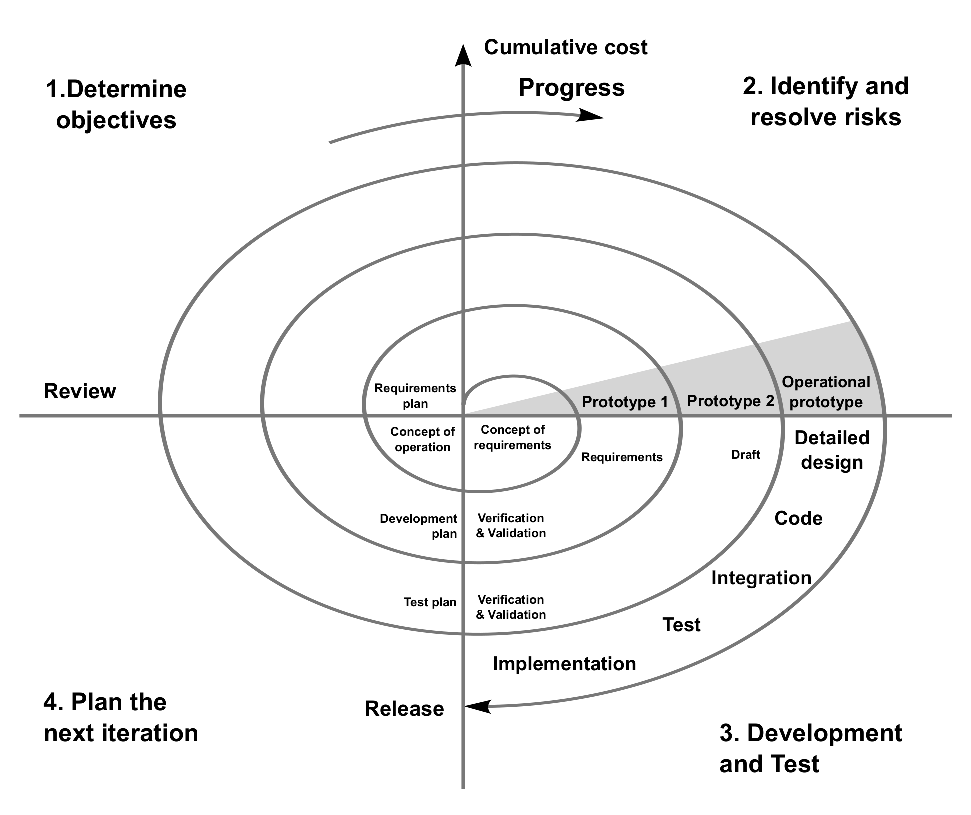
\includegraphics[width=0.7\textwidth]{spiral}
	\caption[The Spiral Model of Software Development]{The Spiral Model of Software Development \citep{boehm_spiral_1988}}
	\label{fig:spiral}
\end{figure}

\subsection{Phases of the Spiral Model}
The phases of the spiral model include the following:

\textit{Determine Objectives, Alternatives and Constraints}

During this phase the objectives for the iteration, and it's alternatives and constraints are investigated.

\textit{Evaluate Alternatives, Identify and Resolve Risks}

The risks involved in the iteration of development are examined, and solutions are found. Additionally, this phase also evaluates the alternatives to the chosen strategy.

\textit{Develop and Verify the Next Level Product}

The development of the product takes place in this phase. For each cycle a different methodology may be used during this phase. For instance, the waterfall model can be used for 

\textit{Plan Next Iteration}

During this phase, with all the information gained from the past cycles, the next iteration is planned.

\subsection{Advantages of the Spiral Model}
The advantages of the Spiral Model are as follows:
\begin{itemize}
	\item It enhances risk avoidance;
	\item A different methodology can be selected for each iteration; and 
	\item It can incorporate the Waterfall, Prototype and Incremental methodologies.
\end{itemize}

\section{Feasibility Studies and Analysis}
Feasibility studies are some preliminary studies undertaken to know whether the project is feasible or not, given a number of circumstances. These studies include; technical, time frame, availability of funds, legal and ethical issues, availability of funds and resources, operation and marketing. With the resource availability, open-source libraries and tools were used throughout the development process, they are always widely available due to their open-source nature. Since this project took the software only approach, it did not include the purchase of certain hardware device, hence the cost for development was down to zero. Other resources like time was heavily considered especially when it could be built; that is, the software had to be functional before the project presentation. Even though it was heavily considered, the time available was suitable enough to develop this software though it interfered with normal day to day activities such as lectures. The feasibility study of this project proved that it was viable.


\section{Requirements Gathering}
A number of questions were asked and answers determined from stakeholders and other interest groups during requirements gathering. Some these questions include:
		\begin{itemize}		
			\item Where is the system going to be used? (Ghana)
			\item Who is going to use the system? (Traveler)
			\item What data should be input into the system? (Text)
			\item What Software Development Life Cycle (SDLC) model to be used? (Spiral)
			\item What type of output information will the system give? (Text and map data)
		\end{itemize}

\subsection{Cost Analysis}
Since this is a software only project we will not concern ourselves with price of hardware.  However, the price of the hardware is directly related to the resources used, which were analysed in the feasibility study. Therefore it is concluded hat this system will depend on the size of data being added to the database and traffic to application.

\subsection{Risk Analysis}
The two main risks involved in this project are the security risks anyone hosting services on the internet will face, and the risk of invalid data or information added by staff or administrator to the database.\\

The first risk is mitigated by limiting the surface area of the system exposed to attackers and by strengthening the components which have been exposed. In this system, the only such component is the search front-end. The search front-end only has read access to the database. Since the information stored therein is public, the only thing a malicious actor can do with this is cause a Denial-of-Service (DoS) attack. Appropriate steps will be taken to mitigate this.\\

The second risk somewhat complex to identify in some cases. Data will pass through several stages of validation and clean up before being made available to the public in order to provide them with the right information.

\subsection{Use Case Diagram}
A Use Case diagram depicts how the users interact with the system. It describes which operations the system can perform and the users as shown in Figure \ref{fig:usecase} below.

\begin{figure}[H]
	\centering
	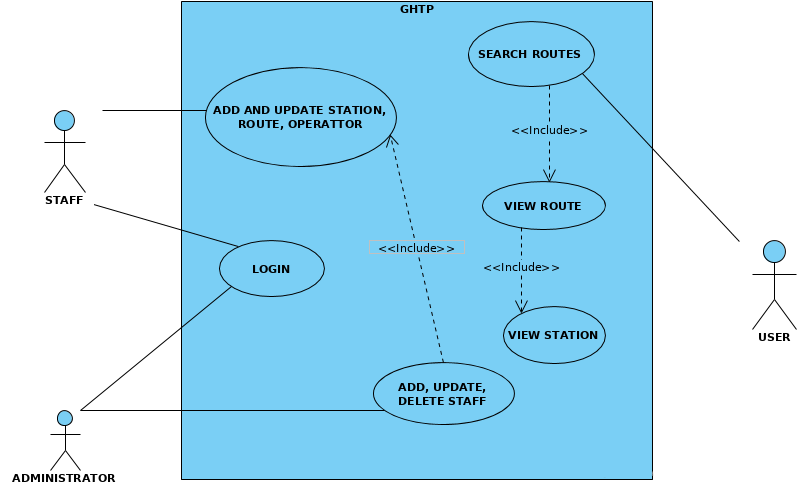
\includegraphics[width=0.9\linewidth]{usecase}
	\caption[Use Case Diangram]{Use Case Diangram}
	\label{fig:usecase}
\end{figure}


\subsection{Activity Diagram}
An activity diagram visually presents a series of actions or flow of control in a system similar to a flowchart or or data flow diagram.

An activity refers to a particular operation of a system. The operations in this system are modeled in to the the activity diagram in Figure \ref{fig:activitydiagram} below.
\begin{figure}[H]
	\centering
	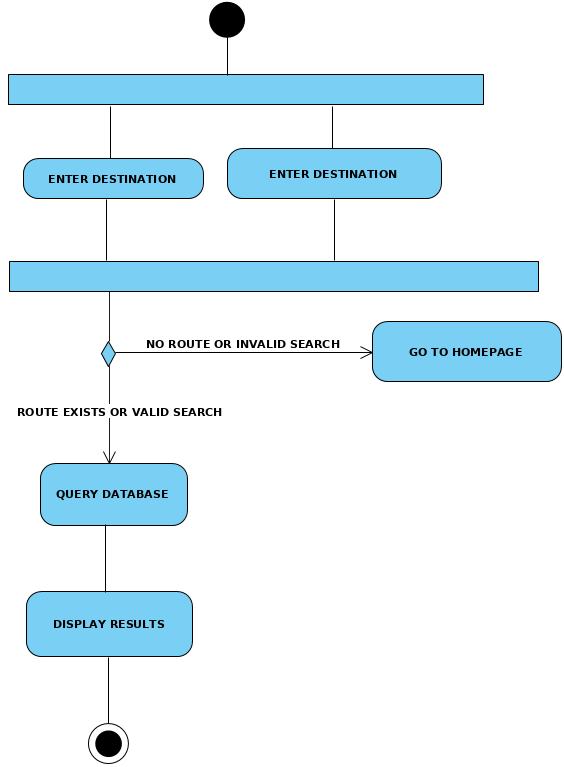
\includegraphics[width=0.7\linewidth]{activitydiagram}
	\caption[Activity Diagram]{Activity Diagram}
	\label{fig:activitydiagram}
\end{figure}

\section{Implementation}
The application is set into operation at the implementation stage. This includes how data is taken by the system, what form of data is taken by the system, where the data is kept, how the data is processed and what form of information is outputted. The first step was to collect and map out transport terminals detailed information in some parts of Ghana; including but not limited to:
\begin{itemize}
	\item Name;
	\item Location (\textit{Town name});
	\item Location (\textit{Longitude and Latitude});
	\item Contacts (\textit{Phone, Email, Website, Operator});
	\item Operators (\textit{STC, GRPTU, VVIP, VIP});
	\item Destinations;
	\item Departure times; and
	\item Vehicle types.
\end{itemize}

The mapped data was uploaded to OpenStreetMap database. After the mapping of the lorry stations, the mapped data was extracted and processed in QGIS before being imported into the projects local PostgreSQL based database.

\begin{figure}[H]
	\centering
	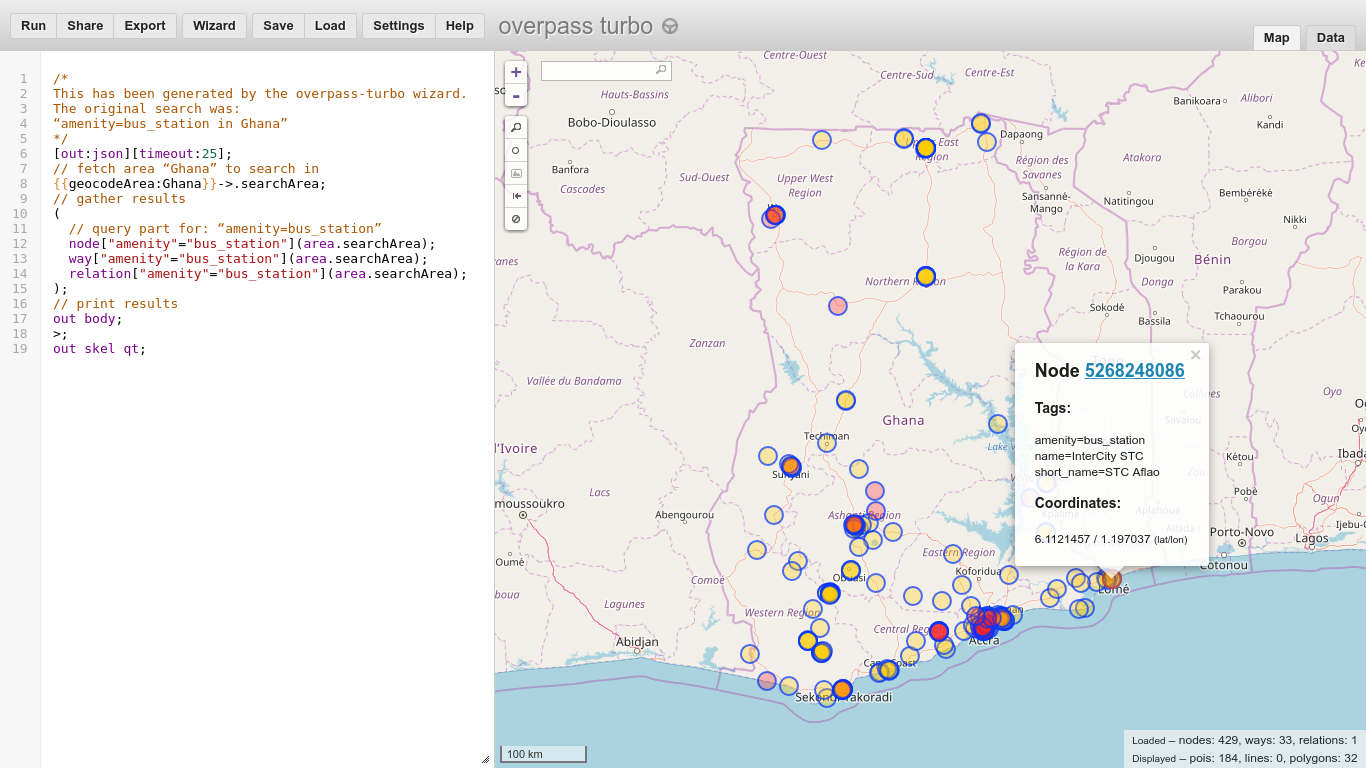
\includegraphics[width=0.9\linewidth]{3/figures/overpass}
	\caption[Extracting mapped data from OpenStreetMap]{Extracting mapped data from OpenStreetMap}
	\label{fig:overpass}
\end{figure}


\subsection{Data Collection}
Data was collected using smartphones and handheld GPS receivers. The following information were collected from the selected lorry stations. Some of these information were collected by survey and crowdsourcing tickets. Some of the data recorded include:
\begin{itemize}
	\item Name;
	\item Operator;
	\item Departure time;
	\item Fares; and 
	\item Available destinations.
\end{itemize}

\begin{figure}[H]
	\centering
	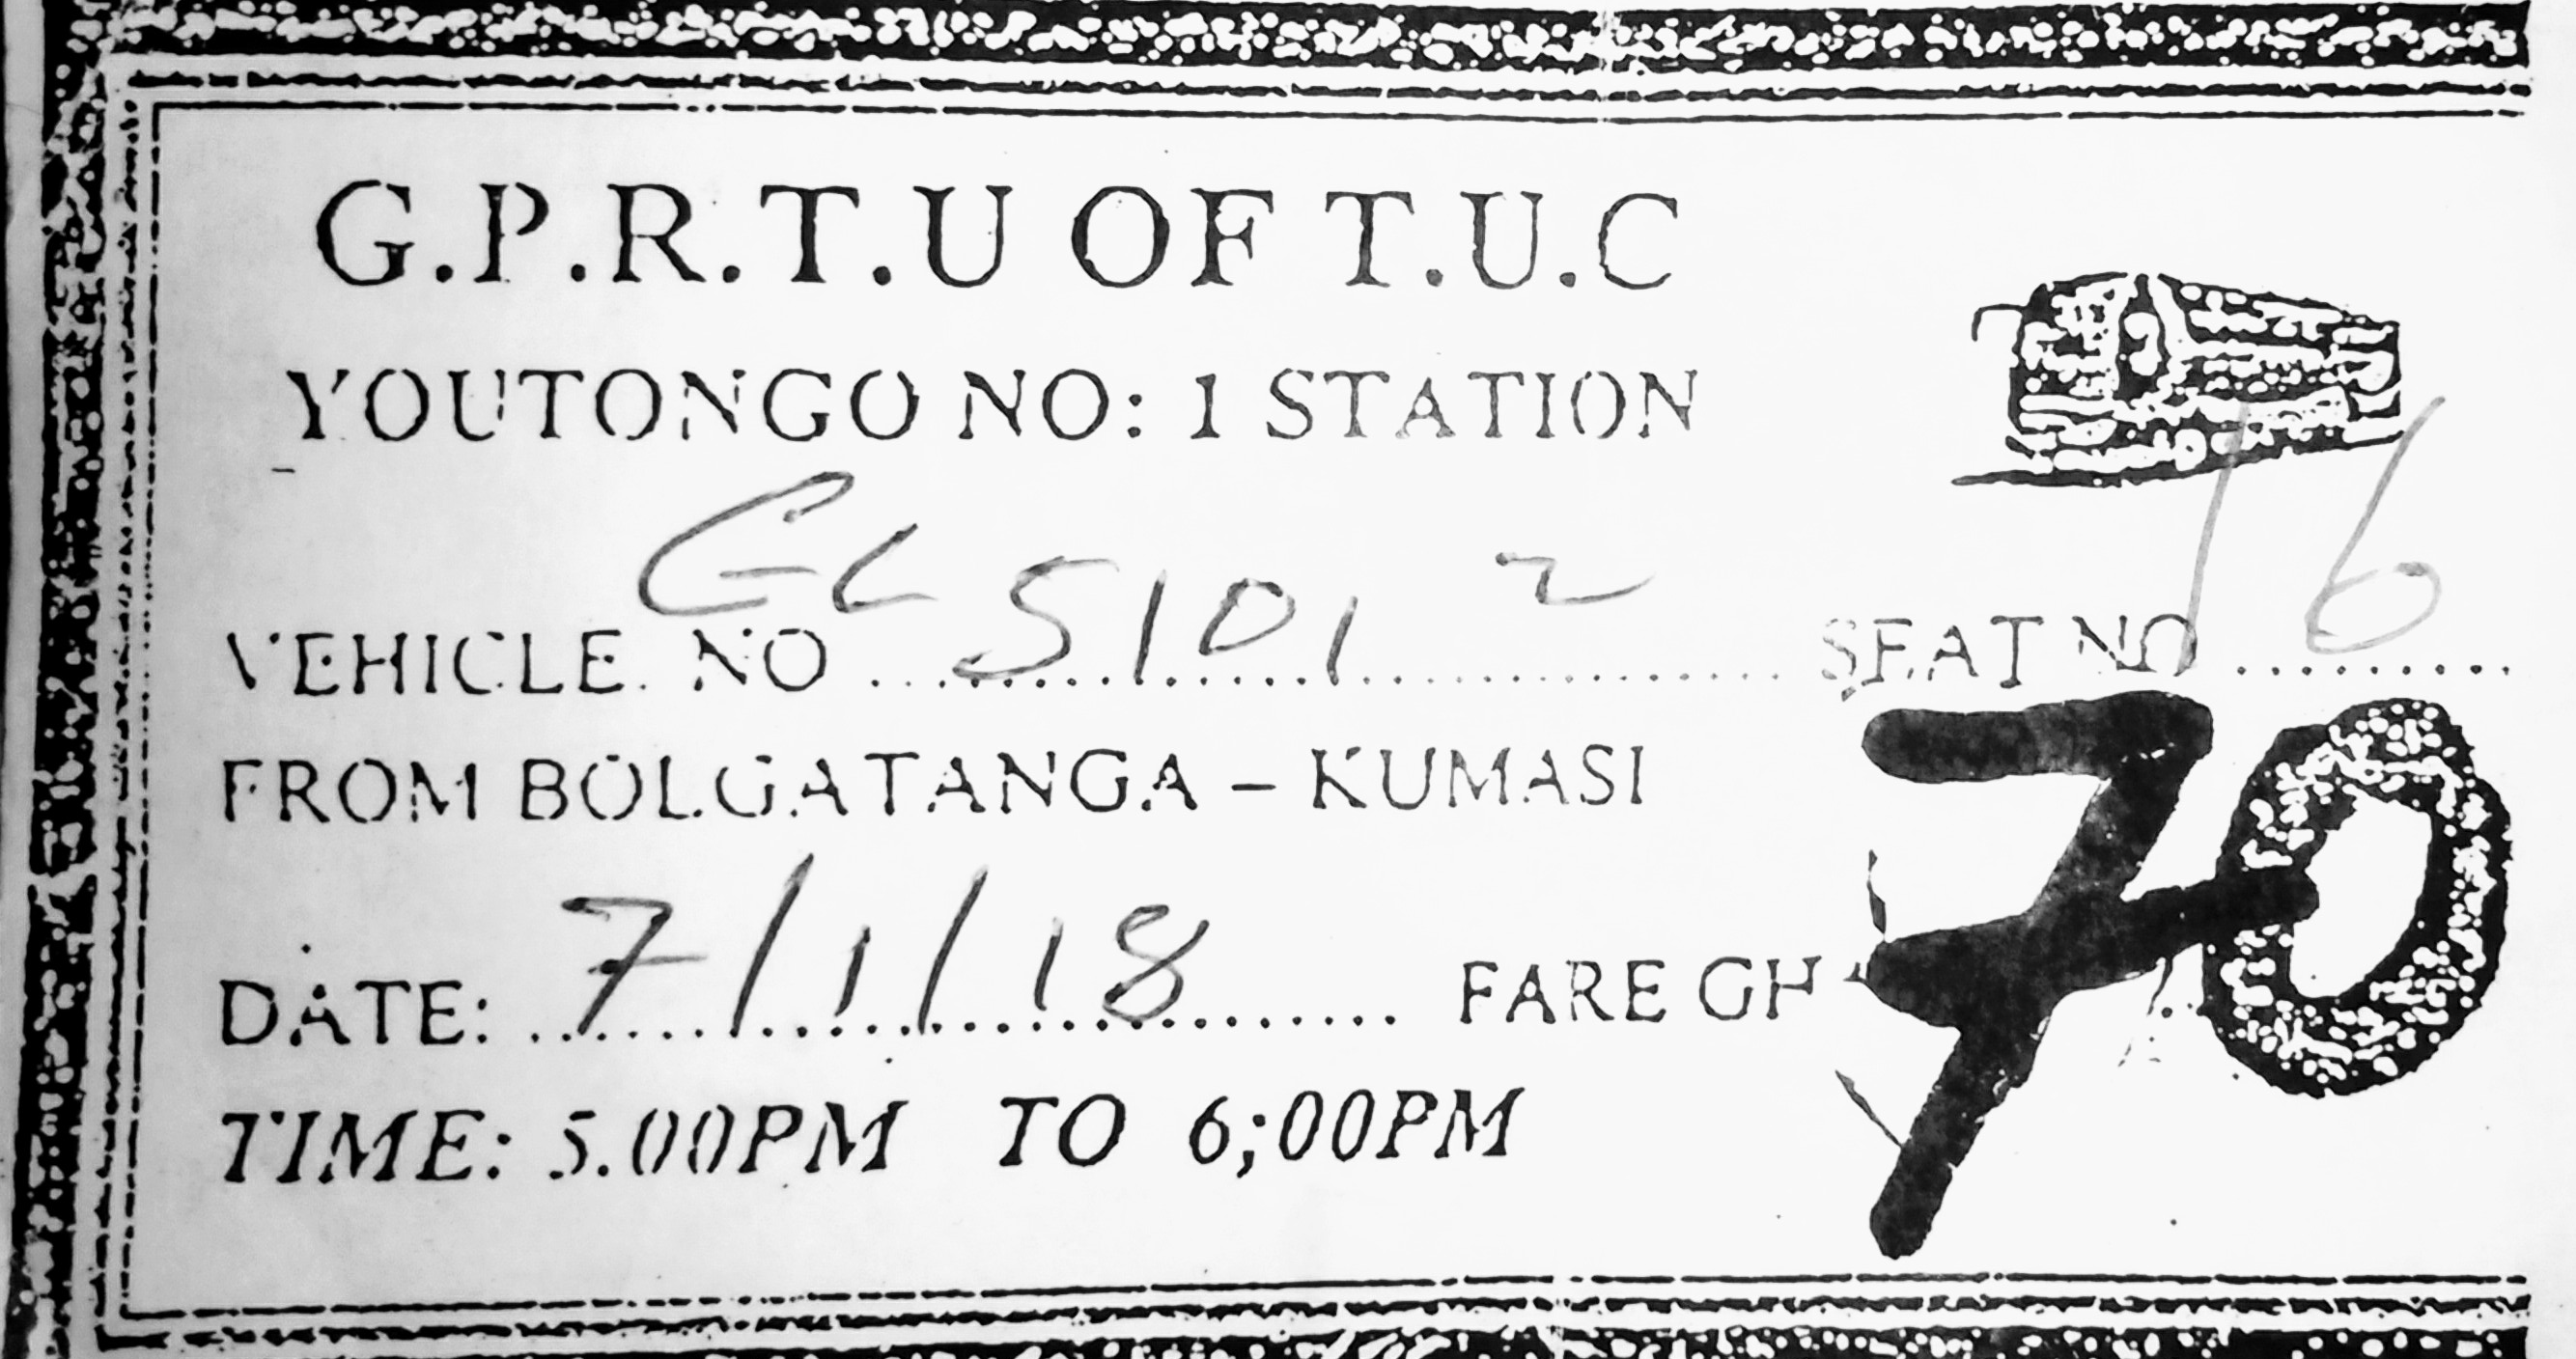
\includegraphics[width=0.6\linewidth]{ticket}
	\caption[Sample bus ticket]{Sample bus ticket}
	\label{fig:ticket}
\end{figure}

\begin{figure}[H]
	\centering
	\includegraphics[width=0.6\linewidth]{schedules}
	\caption[Information available within terminals]{Information available within terminals}
	\label{fig:schedules}
\end{figure}

\subsection{Mapping Transportation Terminals}
The following steps were taken in the mapping out process:
\begin{itemize}
	\item Go to \textit{https://www.osm.org} in a modern web browser such as Firefox of Chromium; 
	\item Searched for town or city where lorry station is to be mapped; 
	\item Area was edited by using JOSM editor as shown in Figure \ref{fig:josm};
	\item Marking out specific areas (buildings, routes (roads, walkways) and the stations are either mapped as points or closed ways (polygons); and
	\item Naming  and describing of points, areas or routes. 
\end{itemize}

\begin{figure}[H]
	\centering
	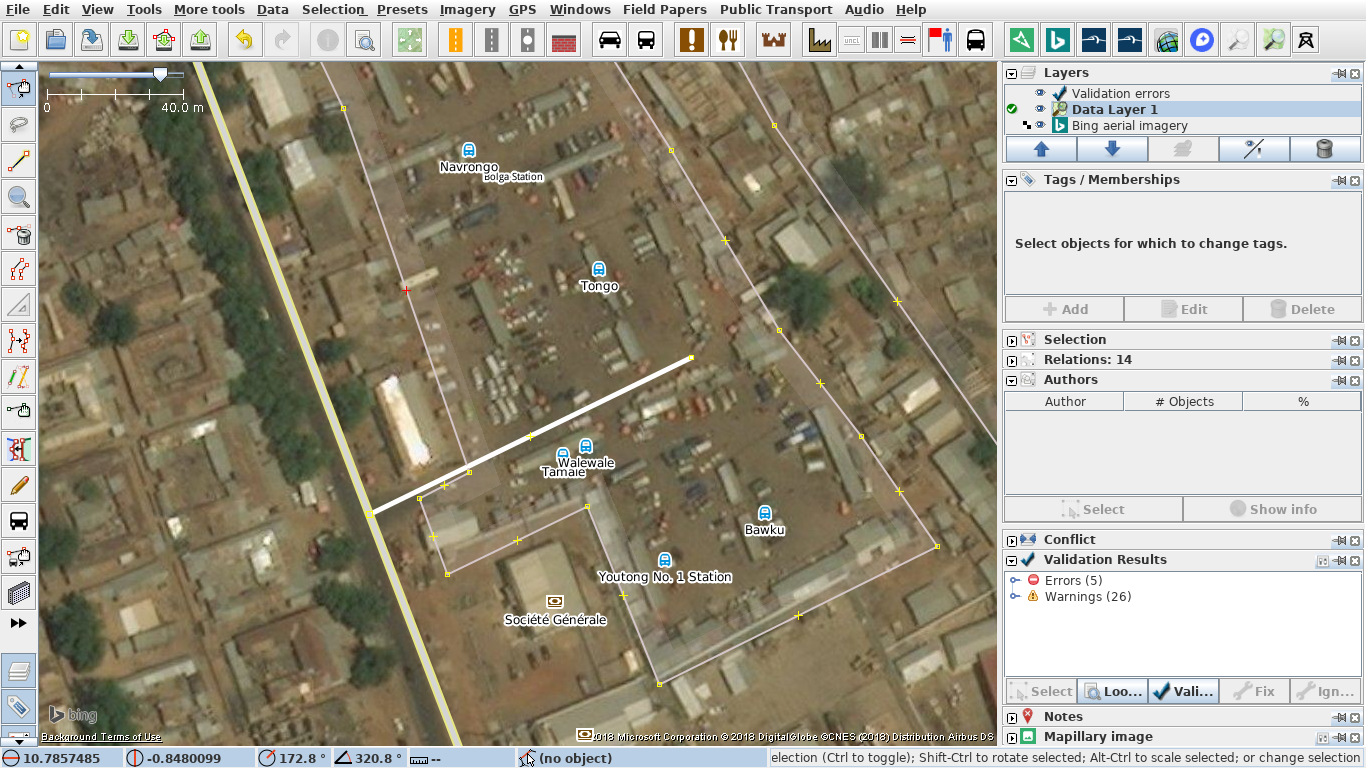
\includegraphics[width=1\linewidth]{josm}
	\caption[Mapping Bus Station into OpenStreetMap]{Mapping Bus Station into OpenStreetMap}
	\label{fig:josm}
\end{figure}

\subsection{Rendering of maps and Routing}
The map showing location various stations was rendered using Leaflet. Routing from departure station is done on the web using the Open Source Routing Machine (OSMRM) Car and OpenStreetMap as a basemap. When the routes and stations locations are accessed from a smartphone with any map based application such as OSMAnd, MAPS.ME, Google Maps, etc they will be prompted to choose an option or else it is opened in a web browser.


% ---------------------------------------------------------------------------
%: ----------------------- end of thesis sub-document ------------------------
% ---------------------------------------------------------------------------

